\section{Linear Transformations, Null Spaces, and Ranges} \label{sec 2.1}

\begin{definition} \label{def 2.1}
Let \(V\) and \(\W\) be vector spaces over the same field \(F\).
We call a function \(\T: V \to \W\) a \textbf{\LTRAN{} from \(V\) to \(\W\)} if, for all \(x, y \in V\) and \(c \in F\), we have
\begin{enumerate}
\item \(\T(x + y) = \T(x) + \T(y)\) and
\item \(\T(cx) = c\T(x)\).
\end{enumerate}
We often simply call \(\T\) \textbf{linear}.
If \(V = \W\), then we call \(\T\) a \textbf{linear operator} on \(V\).
\end{definition}

\begin{remark} \label{remark 2.1.1}
If the underlying field \(F\) is the field of \emph{rational} numbers, then \DEF{2.1} (a) implies (b) (see \EXEC{2.1.38}),
but, in general (a) and (b) are \emph{logically} independent.
See \EXEC{2.1.39} and \EXEC{2.1.40}.
\end{remark}

\begin{remark} \label{remark 2.1.2}
Now you can see why \RMK{2.0.1} assume all vector spaces have common field \(F\), because from \DEF{2.1}, we use the scalar \(c \in F\) on both the input vector \(v \in V\) to get scalar multiplication \(c v\), and the output vector \(\T(v) \in \W\) to get scalar multiplication \(c \T(v)\).
So \(v, \T(v)\) are in \emph{different} vector space \(V\) and \(\W\).
If \(\W, V\) are also over different field, then one of these scalar multiplications will not even be well-defined.
\end{remark}

\begin{additional theorem} \label{athm 2.1}
Given any function \(\T : V \to \W\) (where \(V, \W\) are vector spaces over a command field \(F\)):
\begin{enumerate}
\item If \(\T\) is linear, then \(\T(\OV) = \OW\).
\item \(\T\) is linear if and only if \(\T(cx + y) = c\T(x) + \T(y)\) for all \(x, y \in V\) and \(c \in F\).
\item If \(\T\) is linear, then \(\T(x - y) = \T(x) - \T(y)\) for all \(x, y \in V\).
    (\(x - y\) (or \(\T(x) - \T(y)\)) is just a ``syntactic sugar'' for \(x + (-y)\)(or \(\T(x) + (-\T(y))\)).)
\item \(\T\) is linear if and only if, for \(x_1, x_2, ..., x_n \in V\) and \(a_1, a_2, ..., a_n \in F\), we have
\[
    \T \Big( \sum_{i = 1}^{n} a_i x_i \Big) = \sum_{i = 1}^{n} a_i \T(x_i).
\]
\end{enumerate}
And we generally use (b) to prove that a given function is linear.
\end{additional theorem}

\begin{proof} \ 
\begin{enumerate}
\item
Suppose \(\T\) is linear.
Then
\begin{align*}
    \T(\OV) & = \T(v + (-v)) & \text{for some \(v \in V\)} \\
           & = \T(v) + \T(-v) & \text{by \DEF{2.1}(a)} \\
           & = \T(v) + (-\T(v)) & \text{by \DEF{2.1}(b)} \\
           & = \OW. & \text{by (VS 4) of \(\W\)}
\end{align*}

\item
\(\Longrightarrow\): Suppose \(\T\) is linear.
Then given \(x, y \in V\) and \(c \in F\),
\begin{align*}
    \T(cx + y) & = \T(cx) + \T(y) & \text{by \DEF{2.1}(a)} \\
              & = c\T(x) + \T(y) & \text{by \DEF{2.1}(b)}
\end{align*}

\(\Longleftarrow\):
Suppose given \(x, y \in V\) and \(c \in F\), \(\T(cx + y) = c\T(x) + \T(y)\).
Then in particular, let \(y = \OV\),
\begin{align*}
    \T(cx) & = \T(cx + \OV) & \text{by (VS 3) of \(V\)} \\
           & = \T(cx + y) \\
           & = c\T(x) + \T(y) & \text{by assumption} \\
           & = c\T(x) + \T(\OV) \\
           & = c\T(x) + \OW & \text{by part(a)} \\
           & = c\T(x) & \text{by (VS 3) of \(\W\)}
\end{align*}
And in particular, let \(c = 1\),
\begin{align*}
    \T(x + y) & = \T(1x + y) & \text{by (VS 5) of \(V\)} \\
              & = \T(cx + y) \\
              & = c\T(x) + \T(y) & \text{by assumption} \\
              & = 1\T(x) + \T(y) \\
              & = \T(x) + \T(y) & \text{by (VS 5) of \(\W\)}
\end{align*}
So by \DEF{2.1}, \(\T\) is linear.

\item
Suppose \(\T\) is linear, and \(x, y \in V\).
Then
\begin{align*}
    \T(x - y) & = \T(x + (-y)) & \text{unwrap ``syntactic sugar''} \\
             & = \T(x) + \T(-y) & \text{by \DEF{2.1}(a)} \\
             & = \T(x) + (-\T(y)) & \text{by \DEF{2.1}(b)} \\
             & = \T(x) - \T(y) & \text{add the syntactic sugar back}
\end{align*}

\item
This is immediately true with \DEF{2.1}(a)(b) and induction.
\end{enumerate}
\end{proof}

\begin{example} \label{example 2.1.1}
(Clearly) The function
\[
    \T : \SET{R}^2 \to \SET{R}^2 \text{ by } \T(a_1, a_2) = (2 a_1 + a_2, a_1)
\]
is linear.
\end{example}

\begin{remark} \label{remark 2.1.3}
In general, (informally but trivially,) given \(\T : F^n \to F^m\), if the each component of the output is a linear combination of the components of the input, then \(\T\) is linear.
\end{remark}

\begin{note}
As we will see in \CH{6}, the applications of linear algebra to geometry are wide and varied.
The main reason for this is that \emph{most of the important geometrical transformations are linear}.
Three particular transformations that we now consider are \textbf{rotation, reflection, and projection}.
We leave the proofs of linearity to the reader.
\end{note}

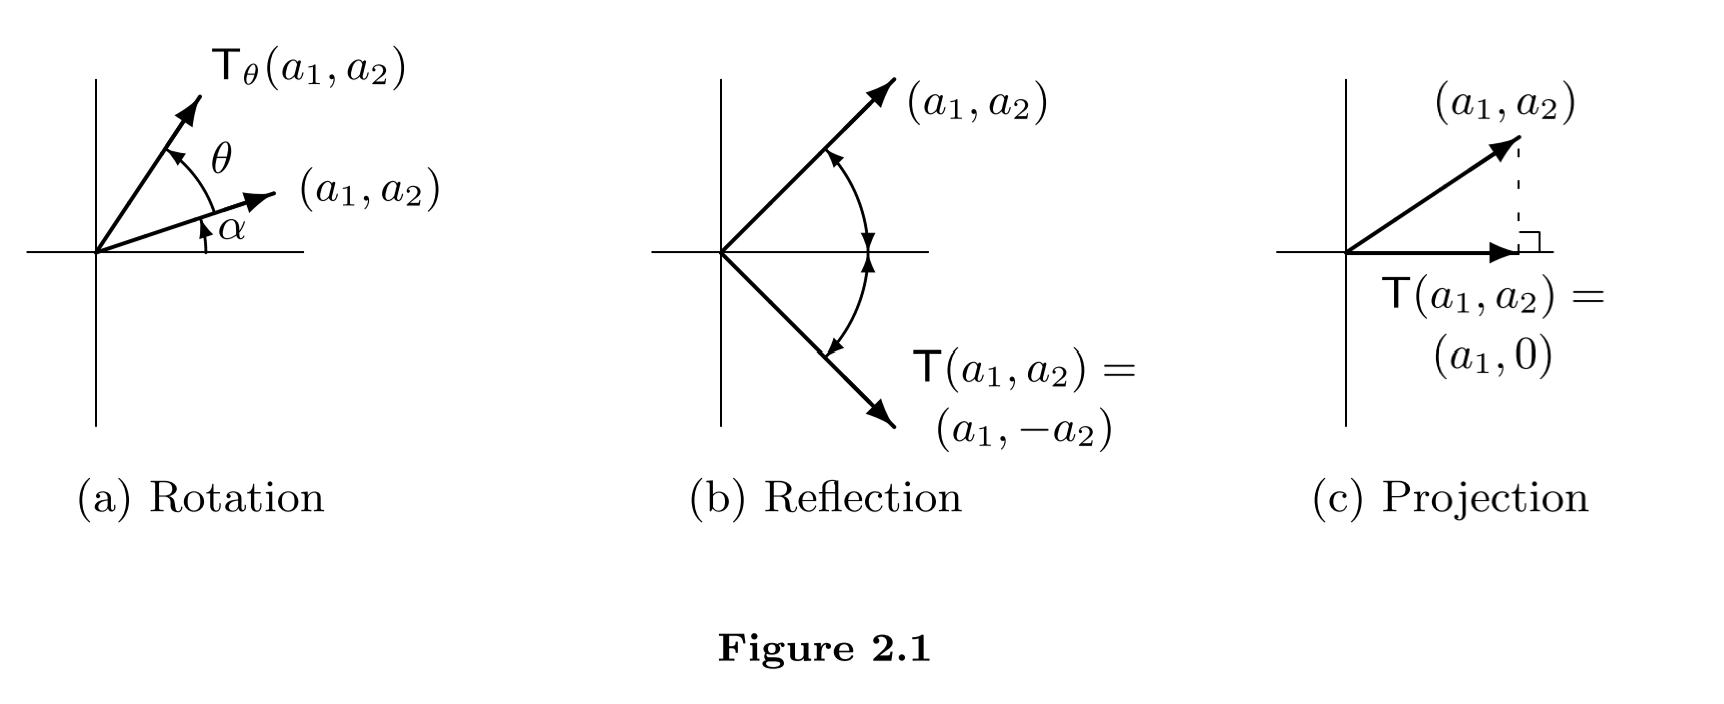
\includegraphics[width=16cm]{images/figure-2-1.png}

\begin{example} \label{example 2.1.2}
For any angle \(\theta\), define \(\T_{\theta} : \SET{R}^2 \to \SET{R}^2\) by the ``rule'':
\(\T_{\theta} (a_1, a_2)\) is the vector obtained by \emph{rotating \((a_1, a_2)\) counterclockwise by \(\theta\)} if \((a_1, a_2) \ne (0, 0)\), and \(\T_{\theta}(0, 0) = (0, 0)\).
Then \(\T_{\theta} : \SET{R}^2 \to \SET{R}^2\) is a \LTRAN{} that is called the \textbf{rotation by \(\theta\)}.

We determine an \emph{explicit formula} for \(\T_{\theta}\).
Fix a nonzero vector \((a_1, a_2) \in \SET{R}^2\).
Let \(\alpha\) be the angle that \((a_1, a_2)\) \emph{makes with the positive \(x\)-axis} (see Figure 2.1(a)),
and let \(r = \sqrt{a_1^2 + a_2^2}\).
Then \(a_1 = r \cos \alpha\) and \(a_2 = r \sin \alpha\).
Also, \(\T_{\theta}(a_1, a_2)\) has length \(r\) and makes an angle \(\alpha + \theta\) with the positive \(x\)-axis.
It follows that
\begin{align*}
    \T_{\theta}(a_1, a_2) & = (r \cos(\alpha + \theta), r \sin(\alpha + \theta)) \\
                         & = (r \cos \alpha \cos \theta - r \sin \alpha \sin \theta,  r \cos \alpha \sin \theta + r \sin \alpha \cos \theta) & \text{by high school algebra} \\
                         & = (a_1 cos \theta - a_2 \sin \theta, a_1 \sin \theta + a_2 \cos \theta). & \text{since \(r \cos \alpha = a_1, r \sin \alpha = a_2\)}
\end{align*}
And by \RMK{2.1.3}, \(\T\) is linear.
\end{example}

\begin{example} \label{example 2.1.3}
Define \(\T : \SET{R}^2 \to \SET{R}^2\) by \(\T(a_1, a_2) = (a_1, -a_2)\).
\(\T\) is called the \textbf{reflection about the \(x\)-axis}.
(See Figure 2.1(b).)
\end{example}

\begin{example} \label{example 2.1.4}
Define \(\T : \SET{R}^2 \to \SET{R}^2\) by \(\T(a_1, a_2) = (a_1, 0)\).
\(\T\) is called the \textbf{projection on the \(x\)-axis} (along \(y\)-axis, see \ADEF{2.2}).
(See Figure 2.1(c).) 
\end{example}

\begin{example} \label{example 2.1.5}
Define \(\T : M_{m \X n}(F) \to M_{n \X m}(F)\) by \(\T(A) = A^\top\), where \(A^\top\) is the transpose of \(A\).
Then \(\T\) is a \LTRAN{} by \EXEC{1.3.3}, since
\begin{align*}
    \T(aA + bB) & = (aA + bB)^\top \\
               & = aA^\top + bB^\top & \text{by \EXEC{1.3.3}} \\
               & = a\T(A) + b\T(B),
\end{align*}
hence \(\T\) is linear by \ATHM{2.1}(b).
\end{example}

\begin{example} \label{example 2.1.6}
Let \(V\) denote the set of all real-valued functions defined on the real line that \emph{have derivatives of every order}.
It is easily shown that \(V\) is a vector space over \(\SET{R}\).
(See \EXEC{1.3.16}.)
Define \(\T : V \to V\) by \(\T(f) = f'\), the derivative of \(f\).
(Note that the input of \(\T\) is itself a function(from \(\SET{R}\) to \(\SET{R}\)); the output of \(\T\) is similar.)
To show that \(\T\) is linear, let \(g, h \in V\) and \(a \in \SET{R}\).
Now
\begin{align*}
    \T(ag + h) & = (ag + h)' \\
              & = ag' + h' & \text{by Calculus} \\
              & = a\T(g) + \T(h).
\end{align*}
So by \ATHM{2.1}(b), \(\T\) is linear.
\end{example}

\begin{example} \label{example 2.1.7}
Let \(V = \mathcal{C}(\SET{R})\), the vector space of all continuous real-valued functions on \(\SET{R}\).
Let \(a, b \in \SET{R}\), \(a < b\).
Define \(\T : V \to \RED{\SET{R}}\) by
\[
    \T(f) = \int_a^b f(t) dt
\]
for all \(f \in V\).
(Note that the input of \(\T\) is a (continuous) function, the output of \(\T\) is the definite integral of that input on the interval \(a, b\).)
Then \(\T\) is a \LTRAN{} because, by Calculus, the definite integral of a linear combination of functions is the same as the linear combination of
the definite integrals of the functions.
\end{example}

\begin{additional definition} \label{adef 2.1}
For vector spaces \(V\) and \(\W\) (over common \(F\)), we define the \textbf{identity transformation} \(\ITRANV: V \to \RED{V}\) by \(\ITRANV(x) = x\) for all \(x \in V\) and the \textbf{zero transformation} \(\TZERO: V \to \W\) by \(\TZERO(x) = \OW\) for all \(x \in V\).
It is clear that both of these transformations are linear.
We often write \(\mathrm{I}\) instead of \(\ITRANV\).
\end{additional definition}

We now turn our attention \emph{to two very important sets associated with \LTRAN{}s}: the \textbf{range} and \textbf{null space}.
The determination of these sets allows us to examine more closely the \emph{intrinsic} properties of a \LTRAN{}.

\begin{definition} \label{def 2.2}
Let \(V\) and \(\W\) be vector spaces, and let \(\T : V \to \W\) be linear.
We define the \textbf{null space} (or \textbf{kernel}) \(\NULLT\) of \(\T\) to be the set of all vectors \(x\) in \(V\) such that \(\T(x) = \OW\);
that is, \(\NULLT = \{ x \in V : \T(x) = \OW \}\).

We define the \textbf{range} (or \textbf{image}) \(\RANGET\) of \(\T\) to be the subset of \(\W\) consisting of all images (under \(\T\)) of vectors in \(V\);
that is, \(\RANGET = \{ \T(x) : x \in V \}\).
\end{definition}

\begin{example} \label{example 2.1.8}
Let \(V\) and \(\W\) be vector spaces, and let \(\ITRANV : V \to V\) and \(\TZERO : V \to \W\) be the identity and zero transformations, respectively. Then \(\NULL(\ITRANV) = \{ \OV \}\), \(\RANGE(\ITRANV) = V\), \(\NULL(\TZERO) = V\), and \(\RANGE(\TZERO) = \{ \OW \}\).
\end{example}

\begin{example} \label{example 2.1.9}
Let \(\T : \SET{R}^3 \to \SET{R}^2\) be the \LTRAN{} defined by \(\T(a_1, a_2, a_3) = (a_1 - a_2, 2a_3)\).
It is left as an exercise to verify that
\[
    \NULLT = \{ (a, a, 0) : a \in \SET{R} \} \text{ and } \RANGET = \SET{R}^2.
\].
\end{example}

\begin{remark} \label{remark 2.1.4}
In \EXAMPLE{2.1.8} and \EXAMPLE{2.1.9}, we see that the range and null space of each of the \LTRAN{}s happen to be a \emph{subspace} (of the codomain and domain, respectively).
The next result shows that this is \emph{true in general}.
\end{remark}

\begin{theorem} \label{thm 2.1}
Let \(V\) and \(\W\) be vector spaces and \(T : V \to \W\) be linear.
Then \(\NULLT\) and \(\RANGET\) are \textbf{subspaces} of \(V\) and \(\W\) (over common \(F\)), respectively.
\end{theorem}

\begin{proof}
We prove \(\NULLT\) and \(\RANGET\) are \textbf{subspaces} of \(V\) and \(\W\) by showing they satisfy the conditions in \THM{1.3}.

Since by \ATHM{2.1}(a), \(\T(\OV) = \OW\), (by \DEF{2.2}) we have that \(\OV \in \NULLT\).
Let \(x, y \in \NULLT\) and \(c \in F\).
Then
\begin{align*}
    \T(x + y) & = \T(x) + \T(y) & \text{since \(\T\) is linear} \\
              & = \OW + \OW & \text{since \(x, y \in \NULLT\)} \\
              & = \OW,
\end{align*}
so by \DEF{2.2}, \(x + y \in \NULLT\);
and
\begin{align*}
    \T(cx) & = c \T(x) & \text{since \(\T\) is linear} \\
           & = c \OW & \text{since \(x \in \NULLT\)} \\
           & = \OW.
\end{align*}
Hence by \DEF{2.2}, \(cx \in \NULLT\), so that by \THM{1.3} \(\NULLT\) is a subspace of \(V\).

Now for \(\RANGET\), because \(\T(\OV) = \OW\), we have that \(\OV \in \RANGET\).
Now let \(x, y \in \RANGE(T)\) and \(c \in F\).
Then there exist \(u\) and \(w\) in \(V\) such that \(\T(v) = x\) and \(\T(w) = y\).
So \(\T(v + w) = \T(v) + \T(w) = x + y\), and \(\T(cv) = c\T(v) = cx\). Thus \(x + y \in \RANGET\) and \(cx \in \RANGET\), so by \THM{1.3}, \(\RANGET\) is a subspace of \(\W\).
\end{proof}

The next theorem provides a method for finding a \emph{spanning set} (\emph{not} necessarily a basis) for the \emph{range} of a \LTRAN{}.
With this accomplished, using the technique of \EXAMPLE{1.6.6} (or \THM{1.9}), it is easy to find a basis, which is a subset of the spanning set, for the \emph{range}.

\begin{theorem} \label{thm 2.2}
Let \(V\) and \(\W\) be vector spaces, and let \(\T : V \to \W\) be linear.
If \(\beta = \{ v_1, v_2 , ..., v_n \}\) is a \emph{basis} for \(V\), then
\[
    \RANGET = \spann(\T(\beta)) =^{\RED{*}} \spann(\{ \T(v_1), \T(v_2), ..., \T(v_n) \}).
\]
(\RED{*} Note that \(\T(\{ v_1, v_2 , ..., v_n \})\) is just a syntactic sugar for \(\{ \T(v_1), \T(v_2), ..., \T(v_n) \}\).)

Also note that we do \emph{not} say \(\T(\beta)\) is a basis for \(\RANGET\);
we just say it is a generating set for \(\RANGET\).
\end{theorem}

\begin{proof} Clearly (by definition of the ``image'' of an input \(v_i\)) \(\T(v_i) \in \RANGET\) for each \(i\).

So \(\{ \T(v_1), \T(v_2), ..., \T(v_n) \} \subseteq \RANGET\).
Because \(\RANGET\) is a \emph{subspace}, by \THM{1.5}(b), \(\RANGET\) contains \(\spann(\{ \T(v_1 ), \T(v_2), ..., \T(v_n) \}) = \spann(\T(\beta))\).

So we have \(\spann(\T(\beta)) \subseteq \RANGET\).

Now suppose arbitrary \(w \in \RANGET\).
Then \(w = \T(v)\) for some \(v \in V\).
Because \(\beta\) is a basis for \(V\), we have
\[
    v = \sum_{i = 1}^n a_i v_i \text{ for some \(a_1, a_2, ..., a_n \in F\)} \MAROON{(1)}.
\]
Since \(T\) is linear, it follows that
\begin{align*}
    w & = \T(v) \\
      & = \T \bigg(\sum_{i = 1}^n a_i v_i \bigg) & \text{by \MAROON{(1)}} \\
      & = \sum_{i = 1}^n a_i T(v_i), & \text{by \ATHM{2.1}(d)} \\
\end{align*}
which is a linear combination of \(\T(\beta)\), hence \(w \in \spann(\T(\beta))\).
So we have \(\RANGET \subseteq \spann(\T(\beta))\).
Hence \(\RANGET = \spann(\T(\beta))\).
\end{proof}

\begin{remark} \label{remark 2.1.5}
It should be noted that \THM{2.2} is true even if \(\beta\) is infinite, that is, \(\RANGET = \spann(\{ \T(v) : v \in \beta \})\).
(See \EXEC{2.1.34}.)
\end{remark}

\begin{example} \label{example 2.1.10}
Define the linear(need to prove, but trivial) transformation \(T : \POLYRR \to M_{2 \X 2}(\SET{R})\) by
\[
    T(f) = \begin{pmatrix}
        f(1) - f(2) &    0 \\
        0           & f(0)
    \end{pmatrix}.
\]
Since \(\beta = \{1, x, x^2\}\) is a basis for \(\POLYRR\), we have
\begin{align*}
    \RANGET & = \spann(\T(\beta)) & \text{by \THM{2.2}} \\
            & = \spann(\{\T(1), \T(x), \T(x^2)\}) & \text{unwrap syntactic sugar} \\
            & = \spann\bigg(\bigg\{
                    \begin{pmatrix}
                        0 & 0 \\
                        0 & 1
                    \end{pmatrix},
                    \begin{pmatrix}
                        -1 & 0 \\
                        0  & 0
                    \end{pmatrix},
                    \begin{pmatrix}
                        -3 & 0 \\
                        0  & 0
                    \end{pmatrix}
                \bigg\}\bigg) \\
            & = \spann\bigg(\bigg\{
                    \begin{pmatrix}
                        0 & 0 \\
                        0 & 1
                    \end{pmatrix},
                    \begin{pmatrix}
                        -1 & 0 \\
                        0  & 0
                    \end{pmatrix}
                \bigg\}\bigg) & \text{by extract subset as basis}
\end{align*}
Thus we have found a basis for \(\RANGET\), and so \(\dim(\RANGET) = 2\).

Now suppose that we want to find a basis for \(\NULLT\).
Note that \(f \in \NULLT\) if and only if \(T(f) = O_{2 \X 2}\), the \(2 \X 2\) zero matrix.
That is, \(f \in \NULLT\) if and only if
\[
    \begin{pmatrix}
        f(1) - f(2) & 0 \\
        0 & f(0)
    \end{pmatrix}
    = \begin{pmatrix}
        0 & 0 \\
        0 & 0
    \end{pmatrix}.
\]
Now express \(f(x) = a + bx + cx^2\) for any \(a, b, c \in \SET{R}\).
If \(f(1) - f(2) = 0\) and \(f(0) = 0\), then we have \(0 = f(1) - f(2) = (a + b + c) - (a + 2b + 4c) = -b - 3c\), or \(b = -3c\);
and \(0 = f(0) = a + 0 + 0 = a\).
So \(f\) must have the form that \(f(x) = 0 + (-3c) x + c x^2 = c(-3x + x^2)\).
Hence \(\NULLT = \{ c(-3x + x^2) : c \in \SET{R} \}\), and trivially the basis is \(\{ -3x + x^2 \}\), hence \(\NULLT\) has dimension \(1\).
\end{example}

\begin{remark} \label{remark 2.1.6}
Note that in \EXAMPLE{2.1.10},
\[
    \dim(\NULLT) + \dim(\RANGET) = 1 + 2 = 3 = \dim(\POLYRR).
\]
In \THM{2.3}, we see that a similar result is \emph{true in general}.
\end{remark}

As in \CH{1}, we ``measure the size'' of a subspace by its dimension.
The null space and range are so important that we \emph{attach special names} to their respective dimensions.

\begin{definition} \label{def 2.3}
Let \(V\) and \(\W\) be vector spaces, and let \(\T : V \to \W\) be linear.
If \(\NULLT\) and \(\RANGET\) are finite-dimensional, then we define the \textbf{nullity} of \(\T\), denoted \(\nullityT\), and the \textbf{rank} of \(\T\), denoted \(\rankT\),
to be the dimensions of \(\NULLT\) -- or \(\dim(\NULLT)\) -- and \(\RANGET\) -- or \(\dim(\RANGET)\) -- respectively.
\end{definition}

\begin{remark} \label{remark 2.1.7}
Reflecting on the action of a \LTRAN{}, we see intuitively that \textbf{the larger the nullity, the smaller the rank}.
In other words, the more vectors that are carried into \(\OW\), the smaller the range.
The same heuristic reasoning tells us that \textbf{the larger the rank, the smaller the nullity}.
This balance between rank and nullity is made precise in the next theorem, appropriately called \textbf{the dimension theorem}.
\end{remark}

\begin{theorem} [Dimension Theorem] \label{thm 2.3}
Let \(V\) and \(\W\) be vector spaces, and let \(\T : V \to \W\) be linear.
If \(V\) is \emph{finite}-dimensional, then
\[
    \nullityT + \rankT = \dim(V).
\]
\end{theorem}

\begin{proof}
Suppose that \(\dim(V) = n, \nullityT = k\), and \(\{ v_1, v_2, ..., v_k \}\) is a basis for \(\NULLT\).
By \CORO{1.11.1}, (since \(\NULLT\) is a subspace of \(V\),) we may extend \(\{ v_1, v_2, ..., v_k \}\) to a basis \(\beta = \{ v_1, v_2, ..., v_k, v_{k +1}, ..., v_n \}\) for \(V\).
We claim that
\[
    S = \{ \T(v_{k + l}), \T((v_{k + 2}), ..., \T(v_n) \}
\]
is a basis for \(\RANGET\).

But first, we need to show that \(\T(v_{k + 1}), ..., \T(v_n)\) are all \textbf{distinct}. (such that \(S\) has \(n - k\) elements.)

For the sake of contradiction, suppose not.
Then there exists \(i \ne j\), \(k + 1 \le i \le n, k + 1 \le j \le n\), such that \(\T(v_i) = \T(v_j)\).
And
\begin{align*}
             & \T(v_i) = \T(v_j) \\
    \implies & \T(v_i) - \T(v_j) = \OW \\
    \implies & \T(v_i - v_j) = \OW & \text{by \ATHM{2.1}(c)} \\
    \implies & v_i - v_j \in \NULLT & \text{by \DEF{2.2}} \\
    \implies & v_i - v_j \in \spann(\{ v_1, ..., v_k \}) \\
    \implies & \{ v_1, ..., v_k, v_i - v_j \} \text{ is \LDP{} } & \text{by \THM{1.7}}
\end{align*}
So we have a \emph{nontrivial} combination \(\OV = a_1 v_1 + ... + a_k v_k + a (v_i - v_j)\).
Note that \(a\) cannot be zero, otherwise one of \(a_1, ..., a_k\) must be nonzero and we have nontrivial representation using \(v_1, ..., v_k\), which contradicts that \(v_1, ..., v_k\) is \LID{}.
But then \(\OV = a_1 v_1 + ... + a_k v_k + a (v_i - v_j) = a_1 v_1 + ... + a_k v_k + a v_i - a v_j\), and that still implies \(\{ a_1, a_2, ..., a_k, a_i, a_j \}\) are \LDP{}, which is a contradiction since it is a subset of a basis (hence \LID{}) of \(\V\).
So \(\T(v_{k + 1}), \T(v_{k + 2}), ..., \T(v_n)\) must be all distinct, so \(S\) really has \(n - k\) elements.

Go back to the consideration of \(S\).
First we prove that \(S\) generates \(\RANGET\).
Using \THM{2.2} (and \(\beta\) is a basis for \(V\)) and \RED{the fact that} \(\T(v_i) = \OW\) for \(1 \le i \le k\), we have
\begin{align*}
    \RANGET & = \spann(\{ \T(v_1), \T(v_2), ..., \T(v_{k}), \T(v_{k + 1}, ..., T(v_n) \}) & \text{by \THM{2.2}} \\
            & = \spann(\{ \OW, \OW, ..., \OW, \T(v_{k + 1}), ..., \T(v_{n}) \}) & \text{using the fact} \\
            & = \spann(\{ \OW, \T(v_{k + 1}), ..., \T(v_{n}) \}) & \text{equal by set theory} \\
            & = \spann(\{ \T(v_{k + 1}), ..., \T(v_{n}) \}) & \text{of course, by \CH{1}} \\
            & = \spann(S).
\end{align*}

Now we prove that \(S\) is \LID{}.
So suppose that
\[
    \sum_{i = k + 1}^n b_i T(v_i) = \OW \text{ for some scalars \(b_{k + 1}, ..., b_n \in F\)}. \MAROON{(1)}
\]
Using the fact that \(\T\) is linear, by \ATHM{2.1}(d), we have
\[
    \T\bigg( \sum_{i = k + 1}^n b_i v_i \bigg) = \OW.
\]
So by \DEF{2.2},
\[
    \sum_{i = k + 1}^n b_i v_i \in \NULLT.
\]
Hence \(LHS\) can be represented as a linear combination of the basis of \(\NULLT\), that is,
\[
    \sum_{i = k + 1}^n b_i v_i = \sum_{i = 1}^k c_i v_i,
\]
hence
\[
    \sum_{i = 1}^k (-c_i) v_i + \sum_{i = k + 1}^n b_i v_i = \OV.
\]
But \(\beta = \{ v_1, ..., v_k, v_{k + 1}, ..., v_n \}\) is known to be the basis of \(V\) (hence is \LID{}), so we have \(c_i\) for \(i = 1, ..., k\) and \(b_i\) for \(i = k + 1, ..., n\) are all equal to zero.
And in particular, \(b_{k + 1} = ... = b_n = 0\).
So by \MAROON{(1)}, \(S\) is \LID{}.

Hence we know \(S\) generates \(\RANGET\) and is \LID{}, so \(S\) is a basis for \(\RANGET\).
Therefore \(\rankT = \#S = n - k\), there for \(\nullityT + \rankT = k + (n - k) = n = \dim(V)\).
\end{proof}

\begin{note}
If we apply the dimension theorem to the \LTRAN{} \(\T\) in \EXAMPLE{2.1.9}, we have that \(\nullityT + 2 = 3\), so \(\nullityT = 1\).
\end{note}

\begin{remark} \label{remark 2.1.8}
The reader should review the concepts of \emph{``one-to-one'' and ``onto''}.
Interestingly, for a \LTRAN{}, both of these concepts are \emph{intimately connected} to the rank and nullity of the transformation.
This is demonstrated in the next two theorems.
\end{remark}

\begin{theorem} \label{thm 2.4}
Let \(V\) and \(\W\) be vector spaces, and let \(\T : V \to \W\) be linear.
Then \(\T\) is one-to-one \emph{if and only if} \(\NULLT = \{ \OV \}\).
\end{theorem}

\begin{proof} \ 

\(\Longrightarrow\): Suppose \(\T\) is one-to-one, we have to show \(\NULLT = \{ \OV \}\).
So let \(x \in \NULLT\), we have to show \(x = \OV\).
By \DEF{2.2}, we have \(\T(x) = \OW\).
But by \ATHM{2.1}(a), \(\T(\OV) = \OW\).
So we have \(\T(x) = \T(\OV)\).
By definition of one-to-one, that implies \(x = \OV\).

\(\Longleftarrow\):
Suppose \(\NULLT = \{ \OV \}\), we have to show \(\T\) is one-to-one.
So suppose arbitrary \(x_1, x_2\) such that \(\T(x_1) = \T(x_2)\), we have to show \(x_1 = x_2\).
Then we have
\begin{align*}
             & \T(x_1) = \T(x_2) \\
    \implies & \T(x_1) - \T(x_2) = \OW \\
    \implies & \T(x_1 - x_2) = \OW & \text{by \ATHM{2.1}(c)} \\
    \implies & x_1 - x_2 \in \NULLT & \text{by \DEF{2.2}} \\
    \implies & x_1 - x_2 = \OV & \text{since \(\NULLT = \{ \OV \}\)} \\
    \implies & x_1 = x_2.
\end{align*}
So by definition, \(\T\) is one-to-one.
\end{proof}

\begin{remark} \label{remark 2.1.9}
\THM{2.4} is true even if \(V\) is \emph{infinite}-dimensional.
\end{remark}

\begin{note}
Observe that \THM{2.4} allows us to conclude that the transformation defined in \EXAMPLE{2.1.9} is not one-to-one since \(\NULLT \ne \{ \OV \}\).
\end{note}

Surprisingly, the conditions of one-to-one and onto are \textbf{equivalent} in an important special case; that is, when the domain and codomain of the \LTRAN{} have the same \emph{finite} dimensions.

\begin{theorem} \label{thm 2.5}
Let \(V\) and \(\W\) be \emph{finite}-dimensional vector spaces \textbf{of equal dimension}, and let \(\T : V \to \W\) be linear.
Then the following are equivalent.
\begin{enumerate}
\item \(\T\) is one-to-one.
\item \(T\) is onto.
\item \(\rankT = \dim(V)\).
\end{enumerate}
\end{theorem}

\begin{proof}
From the dimension theorem \THM{2.3}, we have
\[
    \nullityT + \rankT = \dim(V). \MAROON{(1)}
\]
And we have
\begin{align*}
         & \BLUE{\T \text{ is one-to-one }} \\
    \iff & \NULLT = \{ \OV \} & \text{by \THM{2.4}} \\
    \iff & \nullityT = 0 & \text{by \DEF{2.3}} \\
    \iff & \BLUE{\rankT = \dim(V)} & \text{by \MAROON{(1)}} \\
    \iff & \rankT = \dim(\W) & \text{since \(V\) and \(\W\) have same finite-dimension} \\
    \iff & \dim(\RANGET) = \dim(\W) & \text{by \DEF{2.3}} \\
    \iff & \RED{*} \BLUE{\T \text{ is onto.}}
\end{align*}
So we have shown (a), (b), and (c) are equivalent.

\RED{*}: For the last step, since by \THM{2.1}, \(\RANGET\) is a subspace of \(\W\), and has the same dimension with \(\W\), by \THM{1.11}, \(\RANGET = \W\), which implies \(\T\) is onto.
\end{proof}

\begin{remark} \label{remark 2.1.10}
We note that if \(V\) is \emph{not} finite-dimensional and \(\T : V \to V\) is linear, then \textbf{it does not follow that} one-to-one and onto are equivalent.
(See \EXEC{2.1.15}, \EXEC{2.1.16}, and \EXEC{2.1.21}.)

Note that the \textbf{linearity} of \(\T\) in \THM{2.4} and \THM{2.5} is essential, for it is easy to construct examples of functions from \(\SET{R}\) into \(\SET{R}\) that are not one-to-one, but
are onto, and vice versa.
\end{remark}

\begin{example} \label{example 2.1.11}
Let \(\T : \POLYRR \to \POLYRR\) be the \LTRAN{} defined by
\[
    \T(f(x)) = 2f'(x) + \int_0^x 3f(t) dt.
\]
(Note that integration will make the degree increase by \(1\), so the codomain has one more dimension than domain.)

Now
\begin{align*}
    \RANGET & = \spann(\{ \T(1), \T(x), \T(x^2) \}) & \text{by \THM{2.2}} \\
            & = \spann(\{ 3x, 2 + \frac{3}{2} x^2, 4x + x^3 \}).
\end{align*}
Since \(\{ 3x, 2 + \frac{3}{2} x^2, 4x + x^3 \}\) is \LID{}, \(\rankT = 3\).
Since the dimension of the codomain \(\dim(\POLYRRR) = 4\), \(\T\) is not onto.
From the dimension theorem, \(3 = \dim(\POLYRR) = \nullityT + \rankT = \nullityT + 3\).
So \(\nullityT = 0\), and therefore, \(\NULLT = \{ \OV \}\).
We conclude from \THM{2.4} that \(\T\) is one-to-one.
\end{example}

\begin{example} \label{example 2.1.12}
Let \(\T : F^{\RED{2}} \to F^{\RED{2}}\) be the \LTRAN{} defined by
\[
    \T(a_1, a_2) = (a_1 + a_2, a_1).
\]
It is easy to see that \(\NULLT = \{ \OV \}\);
so by \THM{2.4} \(\T\) is one-to-one.
Hence \THM{2.5} tells us that (since domain and codomain of \(\T\) have same finite dimension,) \(\T\) must be onto.
\end{example}

\begin{note}
In \EXEC{2.1.14}, it is stated that if \(\T\) is linear and one-to-one, then a subset \(S\) (of domain of \(\T\)) is \LID{} if and only if \(\T(S)\) (, a subset of codomain of \(\T\),) is \LID{}.
The next example illustrates the use of this result.
\end{note}

\begin{example} \label{example 2.1.13}
Let \(\T : \POLYRR \to \SET{R}^3\) be the \LTRAN{} defined by
\[
    \T(a_0 + a_1 x + a_2 x^2) = (a_0, a_1, a_2).
\]
Clearly \(\T\) is linear and one-to-one(and onto).
Let \(S = \{ 2 - x + 3x^2, x + x^2, 1 - 2x^2 \}\).
Then \(S\) is \LID{} in \(\POLYRR\) because (by \EXEC{2.1.14} and)
\[
    \T(S) = \{ (2, -1, 3), (0, 1, 1), (1, 0, -2) \}
\]
is \LID{} in \(\SET{R}^3\).
\end{example}

\begin{remark} \label{remark 2.1.11}
In \EXAMPLE{2.1.13}, we \emph{transferred a property} from the vector space of polynomials (with dimension \(3\)) to a property in the vector space of \(3\)-tuples (also with dimension \(3\)).
This technique is exploited more fully later.
(See \SEC{2.4}).
\end{remark}

\begin{note}
\EXEC{2.1.14} 的用意是,你想看一坨向量是否線性獨立,但(可能)很難算,於是你把它們用一個符合一對一的線性函數\ \(\T\) 變換成另一個空間的一坨向量,並且在該空間計算向量是否線性獨立(可能)比較好算;算完後再根據\ \EXEC{2.1.14} 就可知道原本那陀向量是否線性獨立了。
\end{note}

One of the most important properties of a \LTRAN{} is that \textbf{it is completely determined by its action on a basis}.
This result, which follows from the next theorem and corollary, is used frequently throughout the book.

\begin{theorem} \label{thm 2.6}
Let \(V\) and \(\W\) be vector spaces over \(F\), and suppose that \(\{ v_1, v_2, ..., v_n \}\) is a basis for \(V\).
Then given any \(n\) vectors \(w_1, w_2, ..., w_n \in \W\), there \textbf{exists exactly one} \LTRAN{} \(\T : V \to \W\) such that \(\T(v_i) = w_i\) for \(i= 1, 2, ..., n\).
\end{theorem}

\begin{remark} \label{remark 2.1.12}
The purpose of \THM{2.6} is that, if \(V\) and \(\W\) are finite vector spaces, and given any \emph{basis} \(\{ v_1, v_2, ..., v_n \}\) for \(V\), and the ``wanted'' corresponding output \(\{ w_1, w_2, ..., w_n \}\) in \(\W\), we \emph{can always find} a \LTRAN{} from \(V\) to \(\W\) that satisfies the requirement.
Furthermore, the found \LTRAN{} \emph{is unique}.

Hence we can just use a ``mapping'' \(v_1 \to w_1, v_1 \to w_2, ..., v_n \to w_n\) to \emph{identify} the one and only one \LTRAN{}, so this identification is \emph{well-defined}.
And in later sections, we will learn that the ``mapping'' can be represented using \textbf{matrix}!
And that ultimately implies that every \LTRAN{} corresponds to a unique matrix.
\end{remark}

\begin{proof}
Let \(\{ v_1, v_2, ..., v_n \}\) be a basis for \(V\), and let \(w_1, w_2, ..., w_n\) be vectors in \(\W\).

We first prove the existence of \(\T\) such that \(\T\) is linear and \(\T(v_i) = w_i\) for \(i = 1, 2, ..., n\).

So suppose arbitrary \(x \in V\).
Then (since \(\{ v_1, ..., v_n \}\) is a basis for \(V\),)
\[
    x = \sum_{i = 1}^n a_i v_i,
\]
where \(a_1, ..., a_n\) are \textbf{unique} scalars.
Now we prove by construction by defining \(\T\), using this scalars \emph{that depend on \(x\)}:
\[
    \T : V \to \W \text{ by } \T(x) = \T\bigg(\sum_{i = 1}^n a_i v_i\bigg) = \sum_{i = 1}^n a_i w_i. \MAROON{(1)}
\]
Then of course \(\T\) is really a \emph{well-defined} function, since
\BLUE{(1)} it's output is a linear combination of \(\W\)'s vectors, which must be in \(\W\);
\BLUE{(2)} And since for any \(x\) in \(V\), the corresponding scalars \(a_1, ..., a_n\) are \emph{unique}, hence the output of \(\T\) is also unique.
Also note that \MAROON{(1)} is \textbf{not} actually a ``formula'' with ``constant scalars'' \(a_1, ..., a_n\), since \(a_1, ..., a_n\) are determined by (or dependent on) the given \(x\), so they are ``dynamic''.

Then we have to show (a) \(\T\) is linear; (b) \(\T(v_i) = w_i\) for all \(i = 1, ..., n\):
\begin{enumerate}
\item
We will use \ATHM{2.1}(b) to show \(\T\) is linear.
So suppose \(u, v \in V\), and \(d \in F\).
Then (similarly as \(x \in V\),) we may write
\[
    u = \sum_{i = 1}^n b_i v_i \text{ and } v = \sum_{i = 1}^n c_i v_i \MAROON{(2)}
\]
for some (unique) scalars \(b_1, b_2, ..., b_n\) and \(c_1, c_2, ..., c_n\).
Thus
\begin{align*}
    d u + v & = d \sum_{i = 1}^n b_i v_i + \sum_{i = 1}^n c_i v_i \\
            & = \sum_{i = 1}^n (db_i + c_i) v_i \MAROON{(3)} & \text{by rules of finite summation}
\end{align*}
So
\begin{align*}
    \T(du + v) & = \T\bigg( \sum_{i = 1}^n (db_i + c_i) v_i \bigg) & \text{by \MAROON{(3)}} \\
               & = \sum_{i = 1}^n (db_i + c_i) w_i \\
               & \text{\ \ \ \ \ \ (by \MAROON{(1)}; note that now the corresponding} \\
               & \text{\ \ \ \ \ \ \ \ scalars \(a_1, ..., a_n\) in \MAROON{(1)}} \\
               & \text{\ \ \ \ \ \ \ \ are \(d b_1 + c_1, ..., d b_n + c_n\))} \\
               & = d \sum_{i = 1}^n b_i w_i + \sum_{i = 1}^n c_i w_i & \text{by rules of finite summation} \\
               & = d \T\bigg( \sum_{i = 1}^n b_i v_i \bigg) + \T\bigg( \sum_{i = 1}^n c_i v_i \bigg) & \text{again by \MAROON{(1)}} \\
               & = d \T(u) + \T(v), & \text{by \MAROON{(2)}}
\end{align*}
hence \(\T\) is linear.

\item
For \(v_i\) where \(i = 1, ..., n\):
\begin{align*}
    \T(v_i) & = \T(0 v_1 + ... + 1 v_i + ... + 0 v_n) & \text{in particular} \\
            & = 0 w_1 + ... + 1 w_i + ... + 0 w_n & \text{by \MAROON{(1)}, and expand summation} \\
            & = w_i.
\end{align*}
\end{enumerate}
Hence \(\T\) satisfies the two requirements, so the existent part is proved.

Now we have to show \(\T\) is unique.
So suppose \(\U\) is also linear such that \(\U(v_i) = w_i\) for \(i = 1, ..., n\).
We have to show \(\U = \T\);
that is, (by definition of function equality,) we have to show \(\forall x \in V, \U(x) = \T(x)\).

But for each \(x \in V\), where again we represent \(x = \sum_{i = 1}^n a_i v_i\) for unique scalars \(a_1, ..., a_n\) \MAROON{(4)},
\begin{align*}
    \U(x) & = \U\bigg(\sum_{i = 1}^n a_i v_i\bigg) & \text{by \MAROON{(4)}}\\
           & = \sum_{i = 1}^n a_i \U(v_i) & \text{since \(\U\) is linear} \\
           & = \sum_{i = 1}^n a_i w_i & \text{since also \(\U(v_i) = w_i\)} \\
           & = \T\bigg(\sum_{i = 1}^n a_i v_i\bigg) & \text{by \MAROON{(1)}} \\
           & = \T(x). & \text{by \MAROON{(4)}}
\end{align*}
So \(\U = \T\), as desired.
\end{proof}

\begin{note}
There is \href{https://www.youtube.com/watch?v=gAlUekIYKLA&ab_channel=DrPeyam}{another proof} for \THM{2.6}.
\end{note}

\begin{corollary} \label{corollary 2.6.1}
\sloppy Let \(V\) and \(\W\) be vector spaces, and suppose that \(V\) has a finite basis \(\{ v_1, v_2, ..., v_n \}\).
If \(\U, \T : V \to \W\) are linear and \(\U(v_i) = \T(v_i)\) for \(i = 1, 2, ..., n\), then \(\U = \T\).
\end{corollary}

\begin{proof}
Well, since by \THM{2.6} \emph{the} \LTRAN{} that satisfies the mapping \(v_i \to w_i\) for \(i = 1, 2, ... n\) is unique,
and both \(\U, \T\) are linear and satisfy the mapping, hence they are equal to that unique \LTRAN{} hence are equal to each other.
\end{proof}

\begin{example} \label{example 2.1.14}
Let \(\T : \SET{R}^2 \to \SET{R}^2\) be the \LTRAN{} defined by
\[
    \T(a_1, a_2) = (2 a_2 - a_1, 3 a_1),
\]
Then \(\T(1, 2) = (3, 3)\) and \(\T(1, 1) = (1, 3)\), where \(\{ (1, 2), (1, 1) \}\) is a basis for \(\SET{R}^2\).
Now suppose that \(\U : \SET{R}^2 \to \SET{R}^2\) is linear.
If we know that \(\U(1, 2) = (3, 3)\) and \(\U(1, 1) = (1, 3)\), then by \CORO{2.6.1}, \(\U = \T\).
\end{example}
